\section{Hessian zeros, suspension tips, and the contradiction}
\label{cut:section}
\label{sec:cutoffs}

We now justify the integration of the pointwise comparison.  Retain the
original smooth component $\Omega_o\subset S^{m_o}$, with $m_o\in\{4,5\}$,
from Proposition~\ref{red:original-link} and Lemma~\ref{red:nonflat-component}.
Its tensor $T_o$ is not identically zero.  Write
\[
 B_o=\nabla T_o,\qquad w_o=|T_o|,\qquad
 \mathcal Z_o=\{y\in\overline\Omega_o:w_o(y)=0\},\qquad
 \Omega_{o,+}=\Omega_o\setminus\mathcal Z_o.
\]
The tensor $T_o$ is smooth on the compact closure; its norm $w_o$ is
continuous there and smooth where it is positive.  The working domain
$\Omega\subset S^5$ is $\Omega_o$ when $m_o=5$, and its suspension when
$m_o=4$.  On the regular part of this working domain we use the unadorned
notation of Sections~\ref{sec:geometry} and~\ref{sec:flux}.
In particular, $Z$ denotes the flux
vector field, whereas $\mathcal Z_o$ denotes the original Hessian zero set.
Set $M_o=\|w_o\|_{L^\infty(\Omega_o)}$.
We fix
\[
 a=\frac{29}{50},\qquad
 \epsilon_* =\frac{438907}{12000000}>0.
\]
Interior and boundary integrals use their respective spherical volume and
area measures; in the suspension, boundary integrals refer to its regular
side boundary.

\subsection{Weighted integrability on the original component}

\begin{lemma}[Weighted Bochner estimate]\label{cut:weighted-bochner}
The set $\mathcal Z_o$ is a compact subset of $\Omega_o$, and
\begin{equation}\label{cut:weighted-integrability}
 \int_{\Omega_{o,+}}w_o^{2a-2}|B_o|^2\,dV_o<\infty.
\end{equation}
Consequently the function
\begin{equation}\label{cut:original-dominator}
 D_o(y)=
 \begin{cases}
  w_o(y)^{2a}\bigl(1+|B_o(y)|/w_o(y)\bigr)^2,
       &y\in\Omega_{o,+},\\
  0,&y\in\mathcal Z_o,
 \end{cases}
\end{equation}
belongs to $L^1(\Omega_o)$.
\end{lemma}

\begin{proof}
The boundary conclusion of Lemma~\ref{geo:gradient-bound} gives $w_o>0$
at every point of $\partial\Omega_o$.  Compactness and continuity therefore
give a boundary neighborhood on which $w_o$ has a positive lower bound.
The closed set $\mathcal Z_o$ is thus compactly contained in the interior.
If it is empty, $w_o$ has a positive minimum on the whole compact closure,
and \eqref{cut:weighted-integrability} follows immediately from the
boundedness of $B_o$.

Otherwise choose $\eta\in C_c^\infty(\Omega_o)$ with $0\leq\eta\leq1$,
equal to one on an open neighborhood of $\mathcal Z_o$.  For $0<\delta\leq1$
put $W_\delta=w_o^2+\delta$.  Although $w_o$ need not be smooth at its
zeros, $W_\delta$ is smooth and strictly positive.  The identities in
Proposition~\ref{geo:interior-identities} give
\[
 \Delta W_\delta=2m_o w_o^2+2|B_o|^2\geq2|B_o|^2,
 \qquad
 |\nabla W_\delta|^2
 =4|\langle T_o,B_o\rangle|^2
 \leq4W_\delta|B_o|^2.
\]
Set $I_\delta=\int_{\Omega_o}\eta W_\delta^{a-1}|B_o|^2\,dV_o$.
Applying the chain rule to $W_\delta^a$ and integrating twice by parts
against the compactly supported $\eta$ yields
\begin{align*}
 2I_\delta
 &\leq \int_{\Omega_o}\eta W_\delta^{a-1}\Delta W_\delta\,dV_o\\
 &=\frac1a\int_{\Omega_o}(\Delta\eta)W_\delta^a\,dV_o
   +(1-a)\int_{\Omega_o}
       \eta W_\delta^{a-2}|\nabla W_\delta|^2\,dV_o\\
 &\leq\frac1a\int_{\Omega_o}(\Delta\eta)W_\delta^a\,dV_o
       +4(1-a)I_\delta.
\end{align*}
Since
$2-4(1-a)=4a-2=8/25$, this proves the explicit uniform estimate
\begin{equation}\label{cut:absorption}
 \frac8{25}I_\delta
 \leq \frac1a(M_o^2+1)^a\|\Delta\eta\|_{L^1(\Omega_o)}.
\end{equation}
As $\delta\downarrow0$, the nonnegative integrands restricted to
$\Omega_{o,+}$ increase to $\eta w_o^{2a-2}|B_o|^2$ because $a<1$.
Monotone convergence and \eqref{cut:absorption} control that integral.
The compact set $\supp(1-\eta)\subset\overline\Omega_o$ is disjoint from
$\mathcal Z_o$; writing $b_\eta>0$ for the minimum of $w_o$ there, the
remaining integral is bounded by
\[
 \int_{\Omega_{o,+}}(1-\eta)w_o^{2a-2}|B_o|^2\,dV_o
 \leq b_\eta^{2a-2}\|B_o\|_{L^2(\Omega_o)}^2.
\]
Thus all constants in this argument depend only on the fixed original
component and its smooth data, on $a$, and on the chosen interior cutoff
$\eta$, and are independent of $\delta$.  Finally, on $\Omega_{o,+}$,
\[
 D_o\leq2w_o^{2a}+2w_o^{2a-2}|B_o|^2.
\]
The first term is integrable by compactness, and the second by
\eqref{cut:weighted-integrability}.  No measure, dimension, or regularity
property of $\mathcal Z_o$ has been used.
\end{proof}

\subsection{Smooth angular cutoffs and the integrated comparison}

Let $\vartheta\in C^\infty([0,\infty))$ satisfy $0\leq\vartheta\leq1$,
$\vartheta=0$ on $[0,1]$, and $\vartheta=1$ on $[2,\infty)$.  Fix this
profile once and for all, and set
\[
 L_\vartheta=\|\vartheta'\|_\infty,
 \qquad \kappa=2L_\vartheta.
\]
For integers $j\geq3$ define
\begin{equation}\label{cut:cutoffs}
 \alpha_j(y)=\vartheta(jw_o(y)),\qquad
 \xi_j=
 \begin{cases}
  \alpha_j,&m_o=5,\\
  \alpha_j(y)\beta_j(t),\quad
       \beta_j(t)=\vartheta(j\sin t),&m_o=4.
 \end{cases}
\end{equation}
Here $\alpha_j$ is defined to be zero at $\mathcal Z_o$, consistently with
the displayed formula.  It is smooth on $\overline\Omega_o$: near any zero
of $w_o$ it is identically zero, and all its transitions occur where $w_o$
is smooth and positive.  In the suspension, $\beta_j$ vanishes on whole
neighborhoods of both tips.

Figure~\ref{fig:suspension-cutoff} displays the two exclusions made by
the product cutoff in the suspended case. Its transition bands shrink
toward the two tips and the original Hessian zero set. The weighted
estimate above will control the errors produced in all these bands
at once.
\begin{figure}[tbp]
\centering
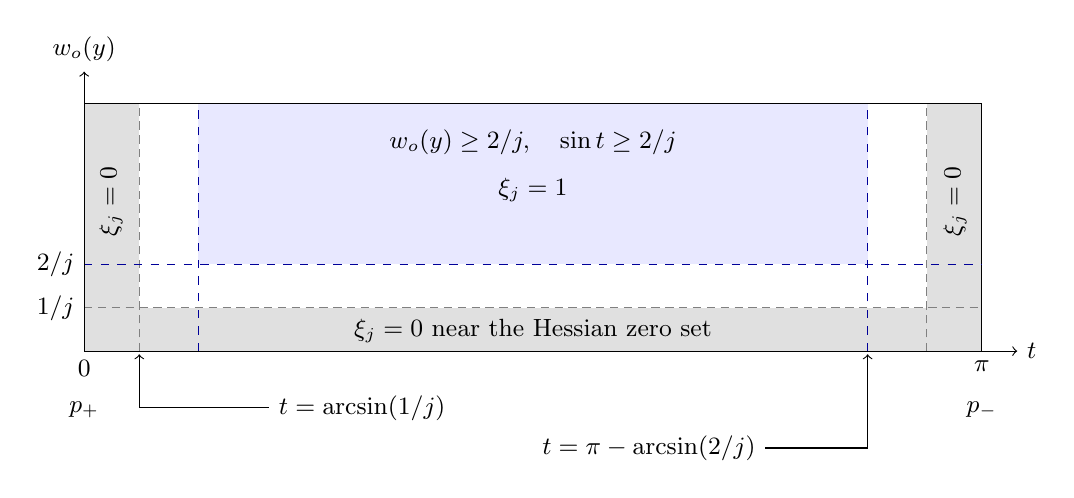
\begin{tikzpicture}[x=1cm,y=1cm,font=\small]
  \fill[gray!24] (0,0) rectangle (11.4,.55);
  \fill[gray!24] (0,.55) rectangle (.7,3.15);
  \fill[gray!24] (10.7,.55) rectangle (11.4,3.15);
  \fill[blue!9] (1.45,1.10) rectangle (9.95,3.15);
  \draw (0,0) rectangle (11.4,3.15);
  \draw[densely dashed,gray] (.7,0)--(.7,3.15);
  \draw[densely dashed,gray] (10.7,0)--(10.7,3.15);
  \draw[densely dashed,gray] (0,.55)--(11.4,.55);
  \draw[dashed,blue!60!black] (1.45,0)--(1.45,3.15);
  \draw[dashed,blue!60!black] (9.95,0)--(9.95,3.15);
  \draw[dashed,blue!60!black] (0,1.10)--(11.4,1.10);
  \node at (5.7,2.05) {$\xi_j=1$};
  \node[align=center] at (5.7,2.65)
    {$w_o(y)\ge 2/j,\quad \sin t\ge 2/j$};
  \node at (5.7,.26) {$\xi_j=0$ near the Hessian zero set};
  \node[rotate=90] at (.34,1.9) {$\xi_j=0$};
  \node[rotate=90] at (11.06,1.9) {$\xi_j=0$};
  \draw[->] (0,0)--(11.85,0) node[right] {$t$};
  \draw[->] (0,0)--(0,3.55) node[above] {$w_o(y)$};
  \node[below] at (0,0) {$0$};
  \node[below] at (11.4,0) {$\pi$};
  \node[left] at (0,.55) {$1/j$};
  \node[left] at (0,1.10) {$2/j$};
  \node[below,align=center] at (0,-.52) {$p_+$};
  \node[below,align=center] at (11.4,-.52) {$p_-$};
  \draw[<-] (.7,-.04)--(.7,-.72)--(2.35,-.72)
    node[right] {$t=\arcsin(1/j)$};
  \draw[<-] (9.95,-.04)--(9.95,-1.23)--(8.65,-1.23)
    node[left] {$t=\pi-\arcsin(2/j)$};
\end{tikzpicture}
\caption{The product cutoff on a suspended component.  The horizontal
variable is the suspension angle in
$\Phi(t,y)=(\sin t\,y,\cos t)$; the two end slices collapse to the
tips $p_+$ and $p_-$.  The vertical variable records the value of
$w_o(y)$, not a coordinate on $\Omega_o$.  Gray regions have
$\xi_j=0$, and the blue region has $\xi_j=1$; the intervening bands
contain the smooth transitions.  The scales are schematic, and no
shape or regularity of the Hessian zero set is represented.}
\label{fig:suspension-cutoff}
\end{figure}


On $\Omega_+=\{x\in\Omega:w(x)>0\}$, use the fields
\[
 h=w^a\sqrt{f(A,p,g)},\qquad
 Z_l=w^{2a}(G_{lijk}X_{ijk}+wM_l+P_l)
\]
constructed in Section~\ref{sec:flux}.  By Lemma~\ref{flux:field-bounds},
there is a fixed $C_F\geq1$ such that
\begin{equation}\label{cut:field-estimates}
 |h|\leq C_Fw^a,\qquad
 |\nabla h|\leq C_Fw^a(1+w+|X|),\qquad
 |Z|\leq C_Fw^{2a}(1+w+|X|).
\end{equation}
The constant depends only on $a$, the dimension $5$, the finitely many
coefficients defining $f,G,M,P$, and the positive lower bound
$f\geq\epsilon_*$.  In particular $C_F$ is independent of the cone,
$w$, $X$, and $j$.

For each fixed $j$, define $v_j=\xi_jh$ and $F_j=\xi_j^2Z$ on $\Omega_+$,
and extend them by zero where $w=0$.  These are smooth on the regular
closure of $\Omega$ and are supported away from the tips when present.
The same neighborhood argument as for $\alpha_j$ proves smoothness of
these extensions; it does not require $h$ or $Z$ themselves to extend
smoothly across $w=0$.  All products below containing one of these cutoff
factors or its derivative are likewise understood to be zero on $w=0$.
The mass $w^{2a}$, whose exponent is positive, has its ordinary value zero
there and involves no normalized tensor.

\begin{lemma}[Integrated comparison]\label{cut:integrated-comparison}
For each fixed $j\geq3$,
\begin{equation}\label{cut:three-errors}
 \epsilon_*\int_\Omega\xi_j^2w^{2a}\,dV
 \leq\int_\Omega\left(
    h^2|\nabla\xi_j|^2
   +2\xi_jh\langle\nabla h,\nabla\xi_j\rangle
   -2\xi_j\langle Z,\nabla\xi_j\rangle\right)\,dV.
\end{equation}
\end{lemma}

\begin{proof}
The interior comparison of Proposition~\ref{flux:interior-comparison}
gives
\[
 \int_\Omega\xi_j^2
       (4h^2+|\nabla h|^2+\epsilon_*w^{2a})\,dV
 \leq\int_\Omega\xi_j^2\diver Z\,dV.
\]
Apply the divergence theorem to the smooth field $F_j$.  In the
suspension one may first truncate the domain inside the two neighborhoods
where $F_j$ vanishes; the artificial end boundaries have zero flux.
On the regular side boundary the outward normal is $-N$.  Thus the
boundary comparison of Proposition~\ref{flux:boundary-comparison},
$N\cdot Z+Hh^2\geq0$, gives
\begin{align*}
 \int_\Omega\xi_j^2\diver Z\,dV
 &=-\int_{\partial\Omega}\xi_j^2\langle N,Z\rangle\,d\sigma
       -2\int_\Omega\xi_j\langle Z,\nabla\xi_j\rangle\,dV\\
 &\leq\int_{\partial\Omega}H(\xi_jh)^2\,d\sigma
       -2\int_\Omega\xi_j\langle Z,\nabla\xi_j\rangle\,dV.
\end{align*}
Corollary~\ref{geo:spherical-stability} applies to $v_j$ and bounds the
boundary integral by
\[
 \int_\Omega\bigl(|\nabla(\xi_jh)|^2+4\xi_j^2h^2\bigr)\,dV.
\]
Expanding the square and canceling the common terms gives
\eqref{cut:three-errors}.
\end{proof}

Every cancellation above is made before removing the angular cutoff.
For fixed $j$ and radial index $k$, the tests $\zeta_k(r)v_j$ from
Corollary~\ref{geo:spherical-stability} have compact support on the
regular Euclidean cone.  First take the variation parameter
$\varepsilon$ to zero on this fixed support; then let $k\to\infty$
in Equation~\eqref{geo:hardy-limit} to obtain the constant $4$.
The smooth extension collar and the allowed variation size may depend
on $j$ and $k$.  We now take $j\to\infty$ only in
Equation~\eqref{cut:three-errors}, which contains the positive mass
and three cutoff errors.  The energy and boundary terms have already
canceled for each fixed $j$.

\subsection{Vanishing of all three errors}

On $\Omega_{o,+}$, differentiation of $\alpha_j$ and
$|\nabla w_o|\leq|B_o|$ give
\begin{equation}\label{cut:original-cutoff-gradient}
 |\nabla_o\alpha_j|
 \leq\kappa\frac{|B_o|}{w_o}.
\end{equation}
To see the constant, wherever $\vartheta'(jw_o)\ne0$ one has
$1<jw_o<2$, so $j\leq2/w_o$; outside this transition region the derivative
is zero.  The same argument gives
\begin{equation}\label{cut:tip-cutoff-gradient}
 |\beta_j'(t)|\leq\frac{\kappa}{\sin t}.
\end{equation}
At every fixed point of $\Omega_{o,+}$, $\alpha_j=1$ and
$\nabla_o\alpha_j=0$ for all sufficiently large $j$.  At every fixed
$t\in(0,\pi)$ the corresponding statements hold for $\beta_j$.

Write $b_o=|B_o|/w_o$ on $\Omega_{o,+}$.  Let $E_{1,j}$, $E_{2,j}$,
and $E_{3,j}$ denote, in order, the three signed integrands on the right
of \eqref{cut:three-errors}.

First suppose $m_o=5$, so $\Omega=\Omega_o$, and set $K_n=1+M_o$.
Since $X=B_o/w_o$,
\[
 1+w+|X|\leq K_n(1+b_o),\qquad
 |\nabla\xi_j|\leq\kappa(1+b_o).
\]
Equations~\eqref{cut:field-estimates} and the preceding bounds give
\begin{equation}\label{cut:nonsuspended-domination}
 |E_{1,j}|+|E_{2,j}|+|E_{3,j}|
 \leq C_F^2(\kappa^2+4K_n\kappa)D_o.
\end{equation}
Indeed the three coefficient bounds are respectively
$C_F^2\kappa^2$, $2C_F^2K_n\kappa$, and $2C_FK_n\kappa$,
and $C_F\geq1$.  The dominator is integrable by
Lemma~\ref{cut:weighted-bochner}.  Each error is eventually zero at
every point of $\Omega_{o,+}$, and is defined to be zero on
$\mathcal Z_o$.  Dominated convergence therefore makes the right side
of \eqref{cut:three-errors} tend to zero.

Now suppose $m_o=4$.  Write $s_t=\sin t$ and use the suspension
coordinates $(t,y)\in(0,\pi)\times\Omega_o$.  The exact formulas in
Proposition~\ref{geo:suspension-data} give
\begin{equation}\label{cut:suspension-scaling}
 w(t,y)=\frac{w_o(y)}{s_t},\qquad
 |B(t,y)|^2
  =\frac{|B_o(y)|^2+3\cos^2(t)w_o(y)^2}{s_t^4},\qquad
 dV=s_t^4\,dt\,dV_o.
\end{equation}
In particular $\Omega_+=(0,\pi)\times\Omega_{o,+}$, and there
\[
 |X|=\frac{\sqrt{b_o^2+3\cos^2t}}{s_t}
       \leq\frac{\sqrt3}{s_t}(1+b_o).
\]
The warped metric gives the exact cutoff identity
\[
 |\nabla\xi_j|^2
 =\alpha_j^2|\beta_j'|^2
   +s_t^{-2}\beta_j^2|\nabla_o\alpha_j|^2,
\]
so \eqref{cut:original-cutoff-gradient}--\eqref{cut:tip-cutoff-gradient}
imply
\begin{equation}\label{cut:suspended-gradient-bounds}
 |\nabla\xi_j|\leq\frac{\kappa}{s_t}(1+b_o),\qquad
 1+w+|X|\leq\frac{K_s}{s_t}(1+b_o),\qquad
 K_s=1+M_o+\sqrt3.
\end{equation}
Multiplying the bounds for the three errors by the volume factor in
\eqref{cut:suspension-scaling} now gives
\begin{equation}\label{cut:suspended-domination}
 s_t^4\bigl(|E_{1,j}|+|E_{2,j}|+|E_{3,j}|\bigr)
 \leq C_F^2(\kappa^2+4K_s\kappa)
          s_t^{2-2a}D_o(y).
\end{equation}
This inequality is initially read on $\Omega_{o,+}$, and both sides are
assigned zero on $\mathcal Z_o$.  Its constant depends only on the
fixed certificate, $a$, $\vartheta$, and $M_o$, and is independent of
$j$, $t$, and $y$.  It also shows explicitly why the original weighted
$|B_o|^2$ estimate suffices: by \eqref{cut:original-dominator},
\[
 s_t^{2-2a}D_o(y)
 \leq 2s_t^{21/25}
       \bigl(w_o^{29/25}+w_o^{-21/25}|B_o|^2\bigr)
 \quad\hbox{on }\Omega_{o,+}.
\]
The right side is integrable with respect to $dt\,dV_o$, because
$21/25>-1$ and \eqref{cut:weighted-integrability} holds.  Every error
is eventually zero at each fixed $(t,y)\in(0,\pi)\times\Omega_{o,+}$.
Dominated convergence applied to \eqref{cut:suspended-domination}
therefore makes the right side of \eqref{cut:three-errors} tend to zero
also in the suspension.

\begin{theorem}\label{cut:exclusion}
The first dimension admitting a nonflat one-homogeneous global minimizer
cannot be $5$ or $6$.
\end{theorem}

\begin{proof}
If the first dimension were $5$ or $6$, the reductions would provide
exactly one of the two working domains just considered.  In either case,
the right side of \eqref{cut:three-errors} tends to zero.  On the original
component, however,
\[
 0<I_o:=\int_{\Omega_o}w_o^{2a}\,dV_o<\infty.
\]
Finiteness follows from boundedness and compactness.  Positivity follows
from $T_o\not\equiv0$ and continuity, which give an open subset of
$\Omega_o$ on which $w_o>0$.  In the nonsuspended case dominated
convergence gives
\[
 \lim_{j\to\infty}\int_\Omega\xi_j^2w^{2a}\,dV=I_o.
\]
In the suspended case \eqref{cut:suspension-scaling} gives instead
\[
 \lim_{j\to\infty}\int_\Omega\xi_j^2w^{2a}\,dV
 = I_o\int_0^\pi(\sin t)^{4-2a}\,dt
 = I_o\int_0^\pi(\sin t)^{71/25}\,dt>0.
\]
Here the dominating mass density is the integrable, everywhere defined
function $(\sin t)^{71/25}w_o^{29/25}$; its value is zero wherever
$w_o=0$.  These strictly positive limits contradict
\eqref{cut:three-errors}, since $\epsilon_*>0$.
\end{proof}

The known lower-dimensional classification gives $d_*\geq5$, and the
dimension-seven globally minimizing example gives $d_*\leq7$, as stated
in Section~\ref{sec:introduction}.  Theorem~\ref{cut:exclusion} excludes the only two
remaining possibilities below $7$.  Hence $d_*=7$, completing the proof
of Theorem~\ref{thm:main}.
